\documentclass[12pt, a4paper]{article}
\pagenumbering{arabic}
\usepackage[utf8]{inputenc}
\usepackage[T1]{fontenc}
\usepackage{geometry}
\usepackage{graphicx}
\graphicspath{{images/}}
\geometry{a4paper}
\usepackage{helvet}
\newcommand\tab[1][1cm]{\hspace*{#1}}
\renewcommand{\familydefault}{\sfdefault}
\setlength{\topmargin}{-2cm}
\setlength{\oddsidemargin}{0cm}
\setlength{\textheight}{24cm}
\setlength{\textwidth}{16cm}
\usepackage{graphicx}
\usepackage{listings}
\usepackage{sectsty}
%Use Helvetica as the sansserif font
\usepackage{helvet}
%Use sffamily for all titles
\allsectionsfont{\sffamily}
\title{THE EXPERIENCE OF SERVICES BY STUDENTS IN NKURUMAH HALL IN MAKERERE UNIVERSITY}
\author{Prepared by Wambogo Brian}
\date{$19^{th} May$ $ 2017$}
\begin{document}
\maketitle
\clearpage
\section{Executive summary(Summary or Abstract)}
The aim of this study was to investigate  the type and quality of services  provided by the hall and the contentment of the students by the services. This report examines the gratification of students by the services provided by the hall ranging from the amenities like (electricity and water), food and security.
\section{Introduction}
Nkurumah hall is a place of a residence within Makerere University that was built in 1954, it was named after the late fist president of Ghana and the founder of Pan African movement called Nkwame Nkurumah. It was first under the management of Northcote hall currently called Nsibirwa hall and it was also referred to as a colony by the residents of Nsibirwa hall. Nkurumah hall only admits and assigns rooms to male students who commonly refer to themselves as activists. The purpose of this study was to find out the impact of the services provided by the hall on the students and to find out the solutions that can be undertaken in order to improve the services for a comfortable better living by the students.
\section{Methodology}
This research was mainly carried out by interviewing resident students in the hall including student leaders. Methods like observation, questionnaires were used to know about the current situation of the hall. This research was also carried out successfully on ground with the help of the ODK collection application that allows one to capture pictures, videos and audios as shown in the picture below.\\
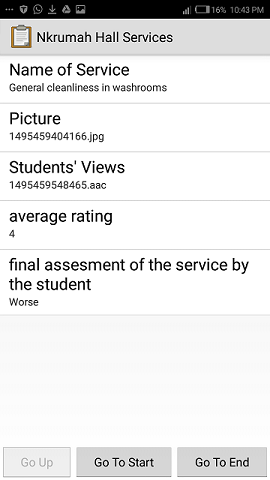
\includegraphics{ODKImage}
\section{Results/Findings}
The research was 85\% successful and the over all assessment of the services is given in percentage by a sample of students as seen in the table below.  . It can clearly be seen from the results that the services are not being delivered to the expectations and satisfaction of the students.


\begin{center}
\begin{tabular}{|| c | c | c | c | c ||}
\hline \textbf{Type of services provided by the hall} & \textbf{Good(\%)}  & \textbf{Average(\%)}  & \textbf{Bad(\%)}  & \textbf{Worse(\%)}\\
[0.5ex]
\hline
\hline Quality of food & 15 & 5 & 10 & 70\\
\hline Rate of water supply & 5 & 15 & 20 & 60\\
\hline General sanitation	  & 10 & 5 & 20 & 65\\
\hline Security at the hall &5 & 10 & 5 & 80\\
[0.5ex]
\hline 
\end{tabular}
\end{center}

\section{Discussion/ Interpretation of Results}
As it can be seen from the table ,services are not generally served to the students’ expectations as 70\% roughly are highly disappointed in the way services are coordinated and provided by the stuff management at Nkurumah hall i.e in the (worse column).





\section{Conclusion}
In general, services in Nkrumah hall are not provided to the expectations of the students and in comparison to the fee that is paid every semester by each student. Student leaders or representatives keep forwarding complaints, but they are not listened to in order to adjust the situation for a better living.
\section{Recommendation}
I recommend that the vice chancellor of Makerere University intervenes to regulate the committee of the halls so that they make proper budgets of the funds paid by students in order to allocate better services to the students.


\clearpage

\Large{\textbf{References}}\\
\normalsize Campusbee.com\\
Students chairman Nkurumah hall (Ahmed Salim)

\end{document}





